    \begin{boxnote}
      \begin{description}
        \item[種類] Article
        \item[閲覧日] 26th May 2025
        \item[キーワード] optomechanical sensing, synthetic magnetism
        \item[文献番号] \cite{PhysRevA.111.053508}
        \item[関連論文] エンタングルメントの論文\cite{PhysRevLett.129.063602},オプトメカニクスのブライトとダーク\cite{lake2020two},超伝導での微小な力の測定\cite{PhysRevLett.128.150501},Synthetic magnetism に関する理論計算\cite{PhysRevLett.129.063602},人工磁場に関する超伝導量子ビットでの測定\cite{massel2012multimode},量子Langevin方程式\cite{PhysRevLett.46.1},実現可能なオプトメカニクス系\cite{eichenfield2009picogram}
      \end{description}
    \end{boxnote}
    \section{行ったこと}
      フォノンホッピングを人工磁場とみなしてオプトメカニクス系を用いて,SQL(Standard quantum limit)を超えた測定の理論提案.
    \section{モデル}
      系のモデルは以下の通り.
      \begin{figure}[H]
        \centering
        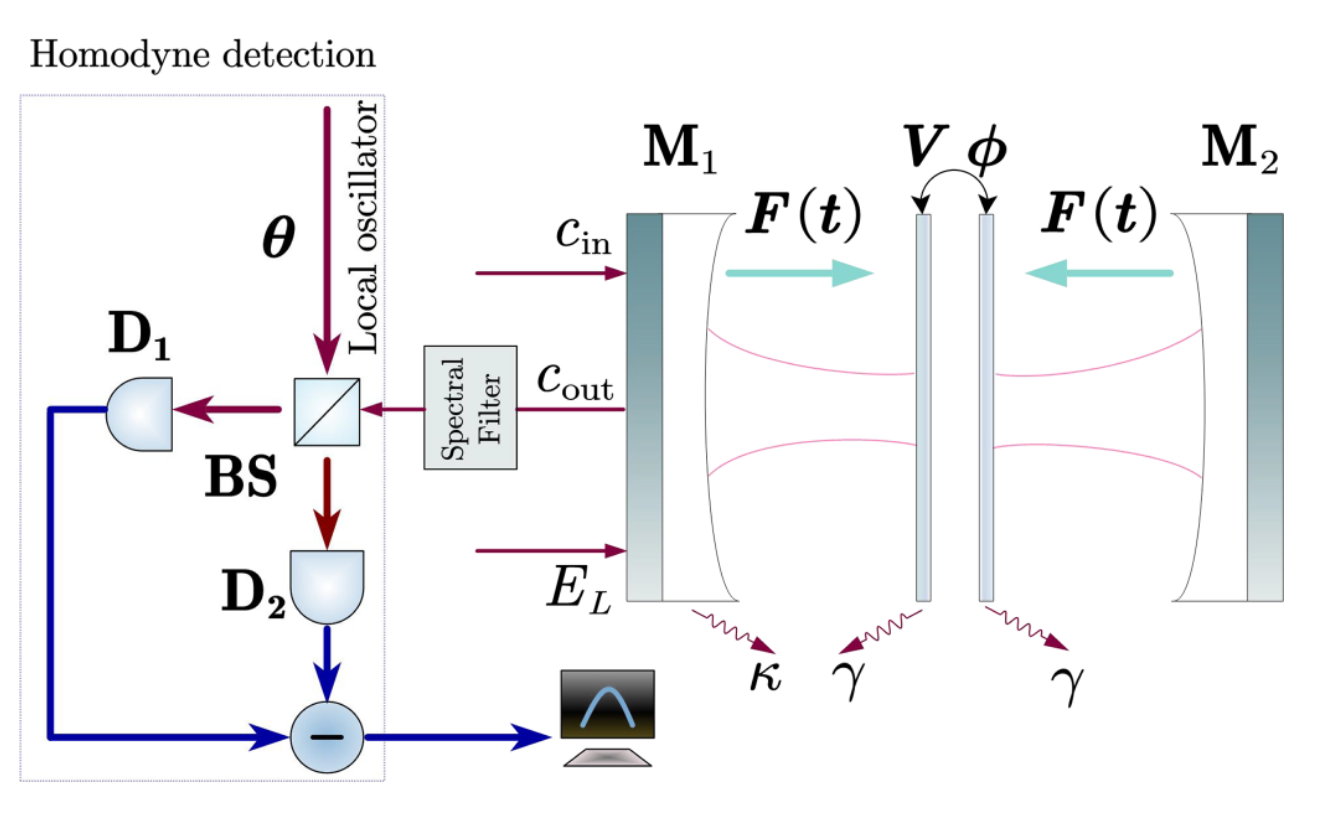
\includegraphics[width = 0.5\linewidth]{./src/Enhancing_optomechanical_force_sensing_utilizing_synthetic_magnetism/1.png}
        \caption{
          系のセットアップ.共振器中に2つの機械振動ミラーがある.共振器内のフォトンのモードが$\hat{c}$,機械振動ミラーのフォノンモードが$\hat{b}$である.
          2つのミラーの結合強度が$F$であり,位相$\phi$が付く.
          系は外部から古典的なコヒーレント光によって駆動されて,強度は$E_{\r{L}}$である.
          共振器にはノイズ$\hat{c}_{\r{in}}$が入る.
          また,共振器からは$\hat{c}_{\r{out}}$の光が出る.
          共振器モードの緩和は$\kappa$であり,フォノンモードの緩和は$\gamma$である.
          検出は,ローカルオシレータ光と$\theta$だけ位相を付けてホモダイン検出を行う.
        }
      \end{figure}
      ドライブする光の周波数$\omega_{\r{L}}$で回転する座標系でのハミルトニアンは,$\omega_{\r{c}}$をフォトンの振動数として,$\Delta \coloneqq \omega_{\r{c}} - \omega_{\r{L}}$とすれば,
      \begin{align}
        \hat{H} = \hbar\Delta\hat{c}^{\dag}\hat{c} +& \hbar\sum_{i = 1, 2} \qty[\omega_{\r{m}}\hat{b}^{\dag}_i\hat{b}_i + g\hat{c}^{\dag}\hat{c}\qty(\hat{b}_i + \hat{b}^{\dag}_i)] \\ 
        +& \hbar V\qty(\e^{\i\phi}\hat{b}^{\dag}_1\hat{b}_2 + \e^{-\i\phi}\hat{b}_1\hat{b}^{\dag}_2) \\ 
        -& x_{\r{ZPF}}F(t)\sum_{i = 1, 2}\qty(\hat{b}_i + \hat{b}^{\dag}_i) + \i\hbar E_{\r{L}}\qty(\hat{c}^{\dag} - \hat{c})
      \end{align}
      と書ける.
      第1項は回転座標系上でのフォトンモード,第2項はフォノンモード,第3項はフォノン・フォトン相互作用,第4項は人工磁場によるフォノンホッピング,第5項は機械振動ミラーのポテンシャル,第6項はレーザ光と共振器モードとの古典的な相互作用.
      さらに,
      \begin{align}
        \hat{X}_i \coloneqq \frac{\hat{b}^{\dag}_i + \hat{b}_i}{\sqrt{2}}, \quad \hat{P}_i \coloneqq \i\frac{\hat{b}^{\dag}_i - \hat{b}_i}{\sqrt{2}}, \quad i = 1, 2
      \end{align}
      とすると,
      \begin{align}
        \hat{H} = \hbar\Delta\hat{c}^{\dag}\hat{c} +& \frac{\hbar\omega_{\r{m}}}{2}\sum_{i = 1, 2}\qty(\hat{X}^2_i + \hat{P}^2_i) + \hbar g\hat{c}^{\dag}\hat{c}\qty(\hat{X}_1 + \hat{X}_2) \\ 
        +& \hbar V\qty[\qty(\cos\phi \hat{X}_1 + \sin\phi \hat{P}_1)\hat{X}_2 + \qty(\cos\phi\hat{P}_1 - \sin\phi\hat{X}_1)\hat{P}_2] \\ 
        +& \i\hbar E_{\r{L}}\qty(\hat{c}^{\dag} - \hat{c}) - F_{\r{ext}}\qty(\hat{X}_1 + \hat{X}_2)
      \end{align}
      と書ける.
      種々の交換関係を用いて量子Langevin方程式を計算すると,
      \begin{align}
        \dot{\hat{c}} &= -(i\Delta + \kappa)\hat{c} - ig\hat{c}(\hat{X}_1 + \hat{X}_2) + E_L + \sqrt{2\kappa}\hat{c}_{\r{in}}\\
        \dot{\hat{X}}_1 &= \omega_{\r{m}}\hat{P}_1 + V \sin\phi\hat{X}_2 + V \cos\phi\hat{P}_2 \\
        \dot{\hat{X}}_2 &= \omega_{\r{m}}\hat{P}_2 - V \sin\phi\hat{X}_1 + V \cos\phi\hat{P}_1 \\
        \dot{\hat{P}}_1 &= -\omega_{\r{m}}\hat{X}_1 - g\hat{c}^{\dagger}\hat{c} - V \cos\phi\hat{X}_2 + V \sin\phi\hat{P}_2 \\
        &\qquad -\gamma\hat{P}_1 + \sqrt{2\gamma}f_{\r{in, 1}} \\
        \dot{\hat{P}}_2 &= -\omega_{\r{m}}\hat{X}_2 - g\hat{c}^{\dagger}\hat{c} - V \cos\phi\hat{X}_1 - V \sin\phi\hat{P}_1 \\
        &\qquad -\gamma\hat{P}_2 + \sqrt{2\gamma}f_{\r{in, 2}}
    \end{align}
    となる.
    平衡点周りで考え,微小変位の記号を省略すると,
    \begin{align}
      \dv{t}\mqty(\hat{X}_{\r{c}} \\ \hat{P}_{\r{c}} \\ \hat{X}_{1} \\ \hat{P}_{1} \\ \hat{X}_{2} \\ \hat{P}_{2}) =
      \mqty(-\kappa & \Delta' & 0 & 0 & 0 & 0 \\
        -\Delta' & -\kappa & -G' & -G' & 0 & 0 \\
        0 & 0 & 0 & V \sin\phi & \omega_{\r{m}} & V \cos\phi \\
        0 & 0 & -V \sin\phi & 0 & V \cos\phi & \omega_{\r{m}} \\
        -G' & 0 & -\omega_{\r{m}} & -V \cos\phi & -\gamma & V \sin\phi \\
        -G' & 0 & -V \cos\phi & -\omega_{\r{m}} & -V \sin\phi & -\gamma)\mqty(\hat{X}_{\r{c}} \\ \hat{P}_{\r{c}} \\ \hat{X}_{1} \\ \hat{P}_{1} \\ \hat{X}_{2} \\ \hat{P}_{2})
        +\mqty(\sqrt{2\kappa}\hat{X}_{\r{in}} \\ \sqrt{2\kappa}\hat{P}_{\r{in}} \\ 0 \\ 0 \\ \sqrt{2\gamma}f_{\r{in, 1}} \\ \sqrt{2\gamma}f_{\r{in, 2}})
    \end{align}
    である.
    以降,
    \begin{align}
      \hat{\bm{u}}(t) \coloneqq\mqty(\hat{X}_{\r{c}} \\ \hat{P}_{\r{c}} \\ \hat{X}_{1} \\ \hat{P}_{1} \\ \hat{X}_{2} \\ \hat{P}_{2}) \quad A \coloneq \mqty(-\kappa & \Delta' & 0 & 0 & 0 & 0 \\
        -\Delta' & -\kappa & -G' & -G' & 0 & 0 \\
        0 & 0 & 0 & V \sin\phi & \omega_{\r{m}} & V \cos\phi \\
        0 & 0 & -V \sin\phi & 0 & V \cos\phi & \omega_{\r{m}} \\
        -G' & 0 & -\omega_{\r{m}} & -V \cos\phi & -\gamma & V \sin\phi \\
        -G' & 0 & -V \cos\phi & -\omega_{\r{m}} & -V \sin\phi & -\gamma) \quad
      \hat{\bm{n}}_{\r{in}} \coloneqq\mqty(\sqrt{2\kappa}\hat{X}_{\r{in}} \\ \sqrt{2\kappa}\hat{P}_{\r{in}} \\ 0 \\ 0 \\ \sqrt{2\gamma}f_{\r{in, 1}} \\ \sqrt{2\gamma}f_{\r{in, 2}})
    \end{align}
    とする.
    改めて,
    \begin{align}
      \dv{\hat{\bm{u}}}{t} = A\hat{\bm{u}} + \hat{\bm{n}}_{\r{in}}
    \end{align}
    である.
    Fourier変換すると,
    \begin{align}
      \hat{\bm{u}} = \qty(-\i\omega\hat{1} - A)^{-1}\hat{\bm{n}}_{\r{in}}
    \end{align}
    と書ける.
    今回はホモダイン検出を行うので,LO項と$\hat{c}_{\r{in}}$の位相差を$\theta$とすると,$\hat{X}_{\r{c}}$のモードの入出力関係式を用いると,
    \begin{align}
      \hat{P}^o(\theta, \omega)\coloneqq A_1\hat{X}^{\r{in}}_{\r{c}} + A_2\hat{P}^{\r{in}}_{\r{c}} + A_3f_{\r{in, 1}} + A_4f_{\r{in, 1}} \label{PhysRevA.111.053508-main-work}
    \end{align}
    として,得られるパワースペクトルは,
    \begin{align}
      S(\omega) \int_{-\infty}^{\infty}\dd{\tilde{\omega}}\frac{\e^{\i\qty(\omega + \tilde{\omega})t}}{4\pi}\ev{\hat{P}^o(\theta, \omega)\hat{P}^o(\theta, \tilde{\omega}) + \hat{P}^o(\theta, \tilde{\omega})\hat{P}^o(\theta, \omega)}
    \end{align}
    によって得られる.
    また,センシングしたい力の信号$S_{\r{F_{ex}}}$に,熱ノイズ$S_{\r{th}}$とその他のノイズ$N^{\theta, \phi}_{\r{add}}$が加わり,応答函数$R^{\theta, \phi}_m$を掛けたものとなる.
    我々は,$R$を大きくして,$N$や$S_{\r{th}}$は小さくしたい.
    途中の計算は追っていない.
    おそらく,\refe{PhysRevA.111.053508-main-work}の計算が主な仕事なのだろう.